\begin{frame}{Theoretical Diagram (tikz)}
\begin{itemize}
    \item Sometimes we might need to draw some theoretical economics diagram, which is painful, I suggest check if there is any similar graph online first. A good source is to check Chiu Yu Ko's website \href{https://sites.google.com/site/kochiuyu/Tikz}{here}, he also has an auto code generator on the bottom of this page. 
\end{itemize}
\begin{figure}
    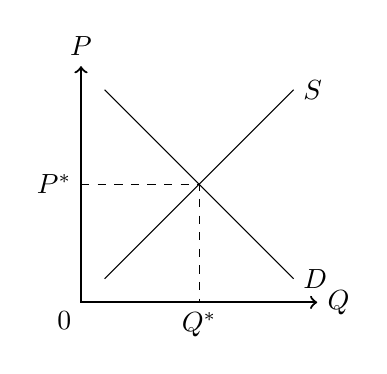
\begin{tikzpicture}[scale=0.3]
\draw[thick,<->] (0,10) node[above]{$P$}--(0,0)--(10,0) node[right]{$Q$};
\node [below left] at (0,0) {$0$};
\node [below] at (5,0) {$Q^*$};
\node [left] at (0,5) {$P^*$};
\draw(1,1)--(9,9) node[right]{$S$};
\draw(1,9)--(9,1) node[right]{$D$};
\draw[dashed](0,5)--(5,5)--(5,0);
\end{tikzpicture}
\caption{supply and demand}\label{figure:supplydemand}
\end{figure}

\end{frame}
% This code uses the tikz package

\begin{frame}{DAG Or Your Mechanism Design (Dagitty)}
    % This code uses the tikz package


% This code uses the tikz package

\begin{tikzpicture}
\node (v0) at (-4.07,1.78) {Overleaf};
\node (v1) at (-1.37,1.02) {LaTex};
\node (v2) at (-2.34,3.71) {Beamer};
\node (v3) at (3.10,1.17) {Python};
\node (v4) at (3.83,-2.60) {STATA};
\node (v5) at (-0.273,-3.83) {R};
\node (v6) at (1.18,-1.15) {Research};
\draw [->] (v0) edge (v1);
\draw [->] (v2) edge (v0);
\draw [->] (v2) edge (v1);
\draw [->] (v1) edge (v6);
\draw [->] (v5) edge (v6);
\draw [->] (v3) edge (v6);
\draw [->] (v4) edge (v6);
\end{tikzpicture}
\end{frame}
